In this section, we discuss the relationship of the various
\textsc{EviL} logics previously developed.  Specifically, we shall
illustrate how the logics developed here provide a network of
conservative extensions.  Hence, we shall be able to complement our
previous upper complexity bounds with lower complexity bounds.

Before proceeding, we will review all of the logics we have developed:

\begin{definition}\label{all-logics}
\begin{description}
  \item[$K$ --] Basic modal logic, with a single modality. We first
    mentioned this logic in \S\ref{sketch}. It is defined in \cite[chapter 4,
    pg. 194]{blackburn_modal_2001}. 
\item[\textsc{EviL} --] The logic axiomatized in Table
  \ref{table:axioms} in \S\ref{evil-axioms}.  It has multiple agents
\item[\textsc{EviL}$^\BM$ --]  The $\BM$ fragment of single agent
  \textsc{EviL}.  This logic was axiomatized in Table
  \ref{table:axiomsII} in \S\ref{subsystems}.
\item[\textsc{EviL}$^\BP$ --]  The $\BP$ fragment of single agent
  \textsc{EviL}.  This logic was axiomatized in Table
  \ref{table:axiomsII} in \S\ref{subsystems}.
\item[$UML$ --] Basic modal logic, with a single modality extended
  with a universal modality.  This means that, in addition to the axioms and rules of the
  basic modal logic $K$, it also possesses the axioms provided in Table
  \ref{table:Uaxioms} from \S\ref{supersystems}.  Note that the
  universal modality axioms of $UML$ are restricted to the basic modal 
  language.  This system is  described in \cite[chapter 7.4]{van_benthem_modal_2010}.
\item[$U$\textsc{EviL}$^\BM$ --] The system \textsc{EviL}$^\BM$
  extended with the axioms provided in Table
  \ref{table:Uaxioms} from \S\ref{supersystems}.
\item[$U$\textsc{EviL}$^\BP$ --] The single agent system \textsc{EviL}$^\BP$
  extended with the axioms provided in Table
  \ref{table:Uaxioms} from \S\ref{supersystems}.
\item[$U$\textsc{EviL} --] \textsc{EviL}
  with multiple agents extended with the universal modality axioms in Table
  \ref{table:Uaxioms} from \S\ref{supersystems}.
\end{description}
\end{definition}

% Using the observed relationships, as well as our 
% previously derived small model properties,  
% we shall present some basic known complexity 
% results for satisfiability in these various logics.

To see how all of these logics inter-relate, we first establish the
following lemma:

\begin{lemma}[$K/UML$ \textsc{EviL} Soundness and Completeness]\label{UML-K-Completeness}
For all $\Gamma$:
\begin{align*}
\Gamma \vdash_K \phi & \iff  \Gamma \Vdash_{\textsc{EviL}} \phi \\
\Gamma \vdash_{UML} \phi & \iff  \Gamma \Vdash_{\textsc{EviL}} \phi 
\end{align*}

For any finite $\Gamma$, given $\Phi$ is infinite:
\begin{align*}
              \Gamma \vdash_K \phi          & \iff  \Gamma \VDash \phi
              \\
              \Gamma \vdash_{UML} \phi          & \iff  \Gamma \VDash \phi
\end{align*}
\end{lemma}
\begin{proof}
In all cases, soundness is trivial so we only need to prove completeness.
Furthermore, we may restrict ourselves to the abstract Kripke
semantics, since result for the concrete semantics follow 
from the abstract results and
 Theorem \ref{UEviL-concrete} from \S\ref{subsystems}.  Finally, we
 shall only show the result for $UML$, since the construction for $K$ is
 similar.

So assume that $\Gamma \nvdash_{UML} \phi$, then there is some model
$\mathbb{M}= \langle W, R, V\rangle$ with a world $w$ such that $\mathbb{M}, w \Vdash \Gamma$
and $\mathbb{M}, w \nVdash \phi$. We need extend this structure to an \textsc{EviL} Kripke
structure.

 It suffices to define
$\sqsupseteq_Y$, $\sqsubseteq_Y$, and $P_Y$ in the following manner:
\begin{align*}
  \sqsupseteq_Y := \sqsubseteq_Y & := id_W = \{(w,v) \in W \times W\
  |\ w = v\}  \\
  P & := \{w \in W \ |\ w R w\} 
\end{align*}

This construction effectively makes every world an island, and ignores
additional agents.  It is straightforward to check that $\langle W,
R, \sqsubseteq, \sqsupseteq, P, V\rangle$ is \textsc{EviL}, and that
it preserves the truth of all $UML$ formulae.
\end{proof}

We may use the various soundness and completeness theorems to see that
the logics defined in Definition \ref{all-logics} give rise to a
network of conservative extensions.  Specifically, the results
employed are:
\begin{bul} 
\item Theorem \ref{evil-completeness} from \S\ref{completely-evil}
\item Theorem \ref{lotsocompleteness} from \S\ref{subsystems}
\item Theorem \ref{universal-completeness} from \S\ref{supersystems}
\item Lemma \ref{UML-K-Completeness} above
\item The (informal) observation that the extension 
of any single agent logic to
  a multi-agent logic is conservative
\end{bul}
  This network is summarized in
Fig. \ref{conservative-extensions}. The network is a Boolean lattice,
where each node corresponds to a set of language features
we have axiomatized.

\begin{figure}[ht]
\begin{center}
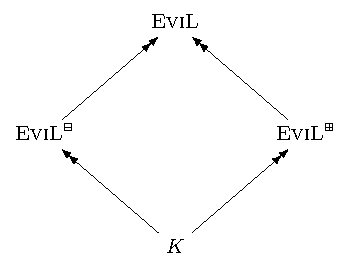
\includegraphics[]{logics/evils.pdf}
\end{center}
\caption{\textsc{EviL} conservative extensions of $K$}
\label{conservative-extensions}
\end{figure}

With the understanding of how these languages inter-relate in terms of
expressivity, we may give complexity bounds on all of the logics discussed:

\begin{lemma}
For any of the logics defined in Definition
\ref{all-logics}, we know their decision problems are $PSPACE$-hard, and can always be
decided in  $3EXPTIME$.

The complexity of the decision problem for all logics extending $UML$
is $EXPTIME$ hard.
\end{lemma}
\begin{proof}
We know that all of the logics can be decided in $3EXPTIME$ by Theorem
\ref{uevil-decidability} from \S\ref{supersystems}, since all of the
systems investigated here are subsystems of U\textsc{EviL}. 

We know all the logics are $PSPACE$ hard, since they all extend basic
modal logic, which is \textsf{PSPACE} complete \cite[chapter
6.3]{van_benthem_modal_2010}.

Similarly, we know all of the logics extending $UML$ are $EXPTIME$
hard, since $UML$ is $EXPTIME$ complete \cite[chapter
7.4]{van_benthem_modal_2010}.
\end{proof}

The network of \textsc{EviL} logics sheds new light on old logics.  An
\textsc{EviL} reading of the minimal modal logic $K$ illustrates that
it is the logic of a single agent justifying their beliefs with
arguments, as we first discussed in \S\ref{sketch}.  $UML$ is a logic where one has background knowledge, the
traditional knowledge studied in epistemic logic.  We may then see
that the other logics correspond to additional epistemic mechanisms 
one may wish to investigate.  This is the \textsc{EviL} perspective on
modal logic:  one begins with concrete intuitions about what is
required to know something, and employs Kripke semantics as a powerful
abstraction on these intuitions.  

This commences our investigations into \textsc{EviL} completeness
theory.

%%% Local Variables: 
%%% mode: latex
%%% TeX-master: "evil_philosophy"
%%% End: 
